\documentclass{article}

\usepackage{graphicx}
\usepackage{tikz}
\usepackage{tikzsymbols}
\usetikzlibrary{calc,patterns,shapes.geometric}
\pagestyle{empty}
\usepackage[margin=0pt]{geometry}
\geometry{papersize={14in,12in}}

\def\centerarc[#1](#2)(#3:#4:#5){\draw[#1] ($(#2)+({#5*cos(#3)},{#5*sin(#3)})$) arc (#3:#4:#5);}

\begin{document}
	\begin{figure}
		\centering
		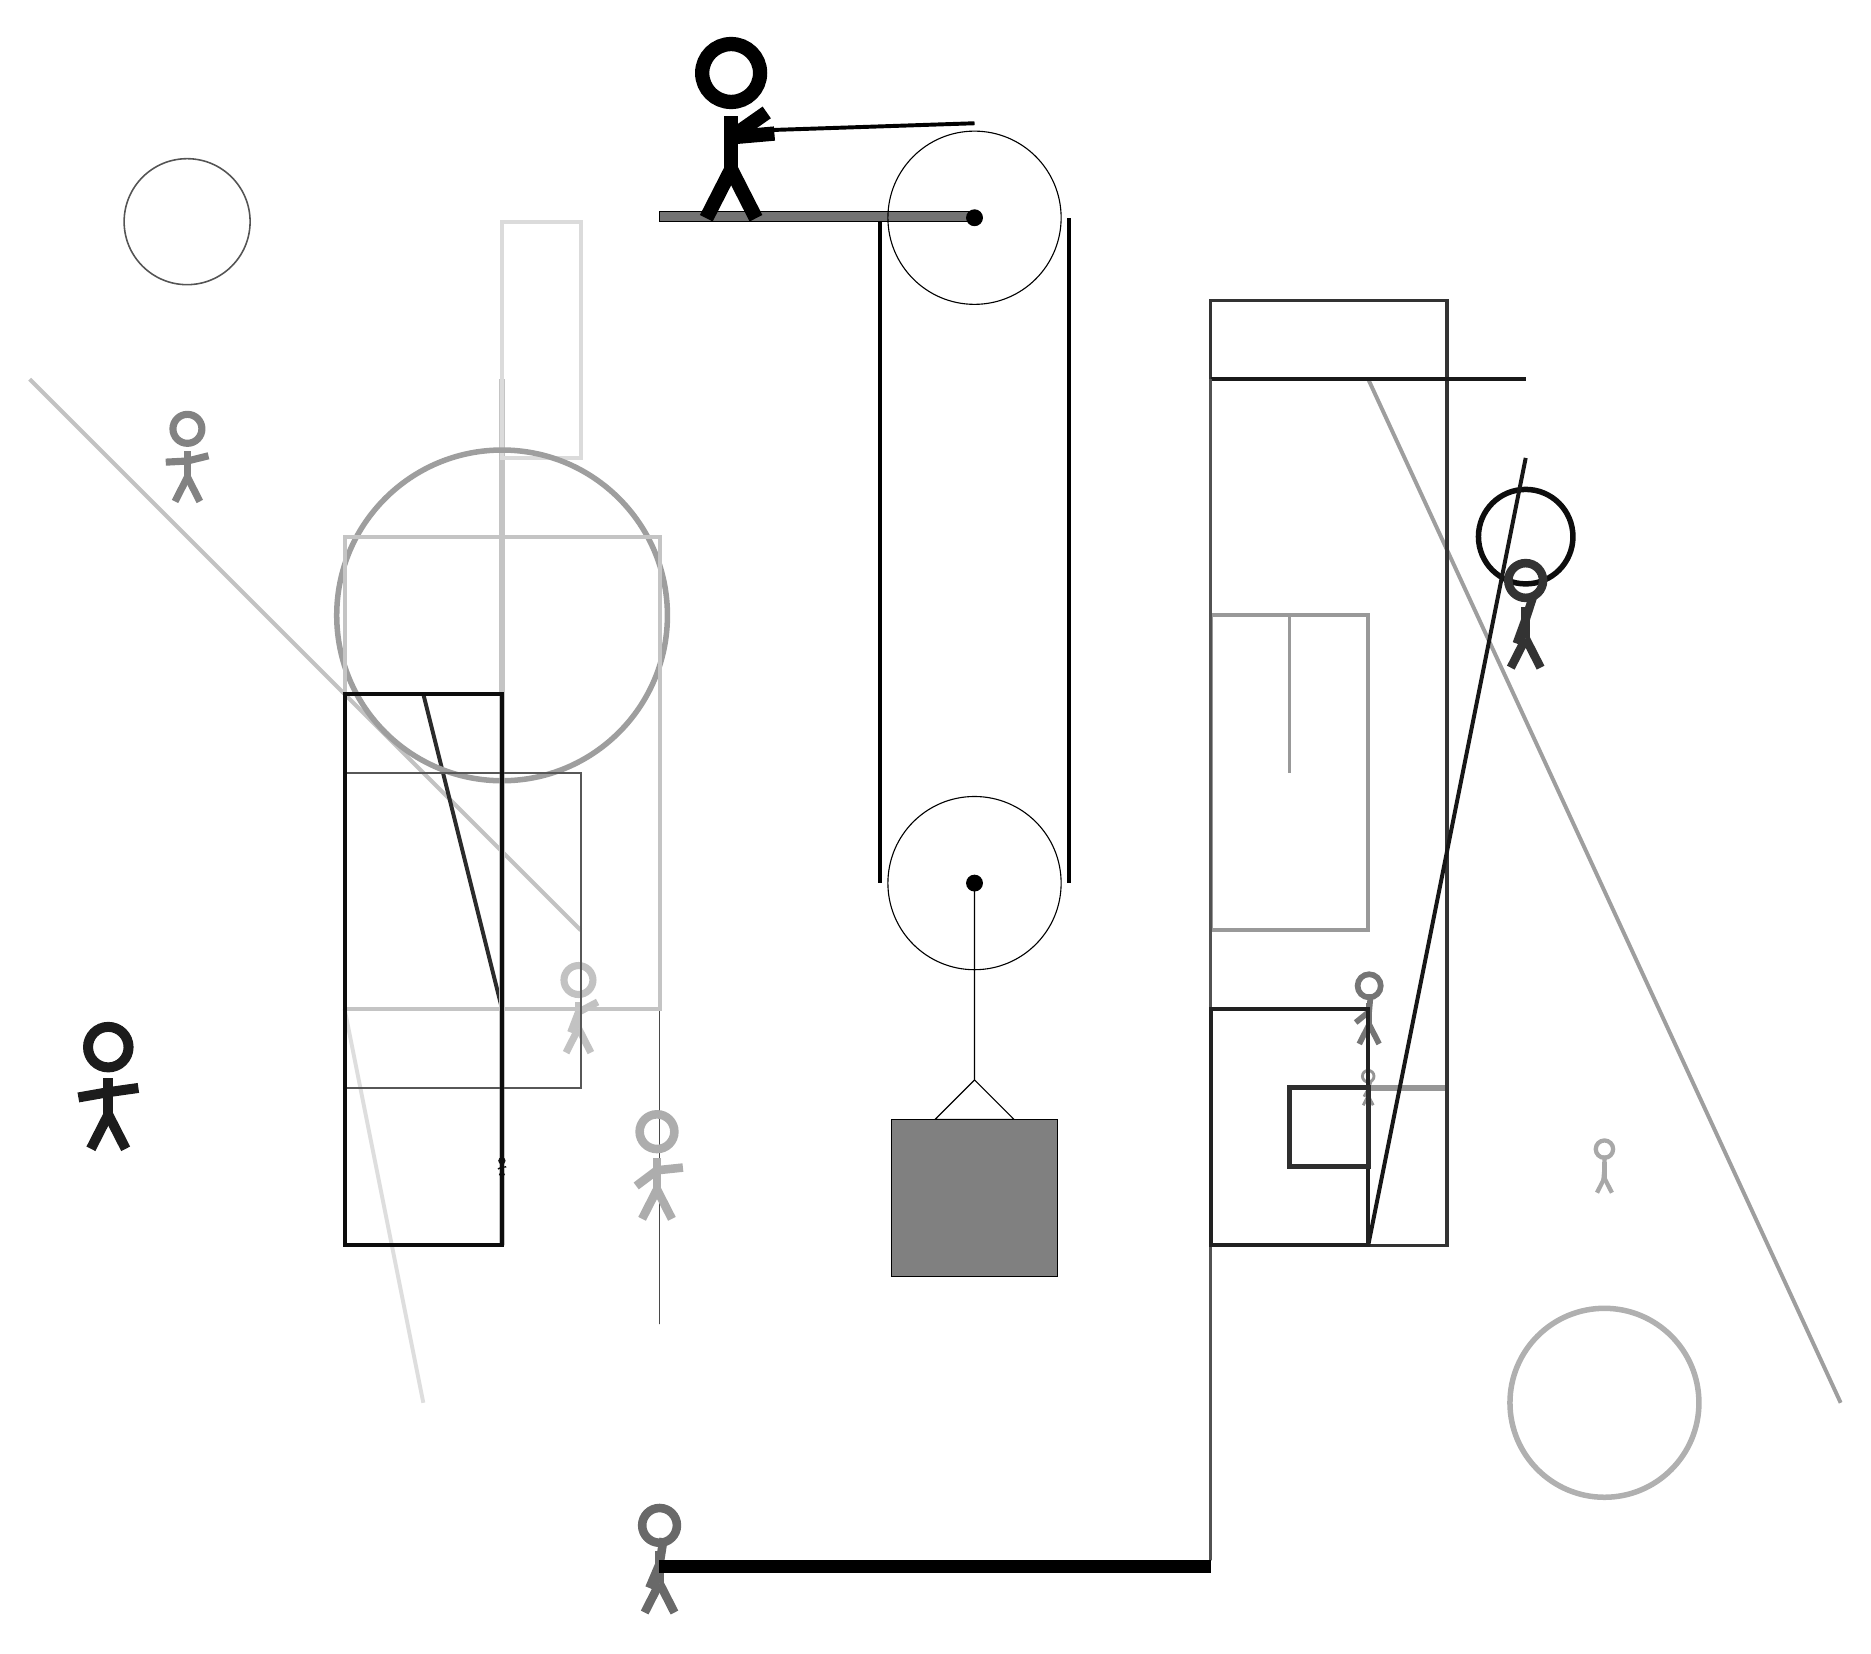
\begin{tikzpicture}
			%%%%% START %%%%%
			
			\draw[fill=black!55] (-2, 14) rectangle (2, 14.125);
			
			\draw (2, 5.6) circle (1.1);
			\draw[fill=black] (2, 5.6) circle (0.1);
			
			\draw (2, 14.05) circle (1.1);
			\draw[fill=black] (2, 14.05) circle (0.1);
			
			\draw[line width=0.5mm, color=black!38](7, 12) -- (13, -1);
			
			\draw[line width=0.5mm, color=black!24](-3, 5) -- (-10, 12);
			\draw [line width=0.6mm, color=black!41](-3, 12) circle (0.0);
			\draw[line width=0.5mm, color=black!83](-4, 4) -- (-5, 8);
			
			\draw[line width=0.5mm, color=black!40] (7, 5) rectangle (5, 9);
			\node[line width=0.6mm, color=black!59] at (-2, -3) {\Strichmaxerl[6][67][81]};
			\draw[line width=0.7mm, color=black!23] (-4, 1) rectangle (-4, 12);
			\draw [line width=0.7mm, color=black!95](9, 10) circle (0.6);
			\node[line width=0.6mm, color=black!49] at (-8, 11) {\Strichmaxerl[5][3][14]};
			\node[line width=0.7mm, color=black!93] at (-4, 2) {\Strichmaxerl[1][24][4]};
			\draw[line width=0.5mm, color=black!14] (-3, 11) rectangle (-4, 14);
			\draw [line width=0.2mm, color=black!67](-8, 14) circle (0.8);
			\draw[line width=0.5mm, color=black!13](-6, 4) -- (-5, -1);
			\draw[line width=0.7mm, color=black!41] (7, 3) rectangle (8, 3);
			\draw[line width=0.2mm, color=black!71] (-2, 0) rectangle (-2, 6);
			\node[line width=0.7mm, color=black!32] at (-2, 2) {\Strichmaxerl[6][37][6]};
			
			\draw [line width=0.7mm, color=black!31](10, -1) circle (1.2);
			\node[line width=0.7mm, color=black!24] at (-3, 4) {\Strichmaxerl[5][69][28]};
			\draw[line width=0.4mm, color=black!80] (5, 13) rectangle (8, 1);
			\node[line width=0.5mm, color=black!42] at (7, 3) {\Strichmaxerl[2][61][70]};
			\draw[line width=0.5mm, color=black!90](5, 12) -- (9, 12);
			
			\draw [line width=0.7mm, color=black!38](-4, 9) circle (2.1);
			
			\node[line width=0.5mm, color=black!34] at (10, 2) {\Strichmaxerl[3][85][89]};
			\node[line width=0.6mm, color=black!54] at (7, 4) {\Strichmaxerl[4][39][85]};
			\draw[line width=0.5mm, color=black!91](9, 11) -- (7, 1);
			\draw[line width=0.5mm, color=black!23] (-2, 4) rectangle (-6, 10);
			\draw[line width=0.2mm, color=black!66] (-3, 7) rectangle (-6, 3);
			\node[line width=0.4mm, color=black!80] at (9, 9) {\Strichmaxerl[6][70][72]};
			\draw[line width=0.4mm, color=black!68] (5, 12) rectangle (5, -3);
			
			\draw[line width=0.5mm, color=black!95] (-4, 8) rectangle (-6, 1);
			\draw[line width=0.5mm, color=black!87] (7, 1) rectangle (5, 4);
			
			\draw[line width=0.3mm, color=black!40] (6, 7) rectangle (6, 9);
			\draw[line width=0.6mm, color=black!82] (6, 3) rectangle (7, 2);
			\node[line width=0.4mm, color=black!89] at (-9, 3) {\Strichmaxerl[7][10][8]};
			
			\draw (2, 5.6) -- (2, 3.1) -- (1.5, 2.6) -- (2.5, 2.6) -- (2, 3.1);
			\draw[fill=black!50] (0.95, 2.6) rectangle (3.05, 0.6);
			
			\draw[line width=0.5mm] (0.8, 14) -- (0.8, 5.6);
			\centerarc[line width=0.5mm](2, 5.6)(180:360:1.2000000000000002);
			\draw[line width=0.5mm](3.2, 5.6) -- (3.2, 14.05);
			\centerarc[line width=0.5mm](2, 14.05)(0:90:1.2000000000000002);
			\draw[line width=0.5mm](2, 15.25) -- (-1, 15.15);
			
			\node at (-1, 15.15) {\Strichmaxerl[10][-175][35]};
			
			\draw[fill=black] (-2, -3) rectangle (5, -3.15);
			
			%%%%% END %%%%%
		\end{tikzpicture}
	\end{figure}	
\end{document}